\documentclass[aip,cha,reprint]{revtex4-2}
\usepackage[T1]{fontenc}
\usepackage[utf8]{inputenc}
\usepackage{amsmath,amssymb,bm,booktabs,graphicx,siunitx}
\usepackage[nameinlink,capitalize,noabbrev]{cleveref}
\usepackage{xr}
\externaldocument[MAIN-]{Chaos_Floquet_SyntheticFlux}
\sisetup{detect-all}

\newcommand{\dd}{\,\mathrm{d}}
\newcommand{\Tr}{\operatorname{Tr}}

\begin{document}
\title{Supplementary Material: physical anchoring and matched measurement-Fisher reference for dissipative optomechanics with synthetic flux}
\author{Stella Rolande Mbokop Tchounda and Carolle Tchodimou}
\affiliation{Department of Physics, Faculty of Science, University of Yaound\'e I, P.O. Box 812, Yaound\'e, Cameroon}

\author{Philippe Djorwe}
\affiliation{Department of Physics, Faculty of Science, University of Ngaound\'er\'e, P.O. Box 454, Ngaound\'er\'e, Cameroon}

\author{Sifeu Takougang Kingni}
\affiliation{Department of Mechanical, Petroleum and Gas Engineering, National Advanced School of Mines and Petroleum Industries, University of Maroua, P.O. Box 46, Maroua, Cameroon}

\author{Serge Guy Nana Engo}
\affiliation{Department of Physics, Faculty of Science, University of Yaound\'e I, P.O. Box 812, Yaound\'e, Cameroon}
\email{serge.nana-engo@facsciences-uy1.cm}

\maketitle

\section{Normalization and anchor selection}

The main text uses a rotating-frame Hamiltonian normalized to a reference
mechanical frequency $\omega_m$, so that all rates and couplings are reported as
dimensionless ratios $x/\omega_m$. A physically anchored reference set is obtained by
fixing $\omega_m$ from a device with gigahertz mechanical modes and optically mediated
phonon coupling, and by reading the damping, decay, and coupling rates from the same
platform. The two primary anchors are:

\begin{itemize}
\item \textbf{Mayor \emph{et al.}~\cite{Mayor2025}}: a silicon two-dimensional optomechanical
crystal with mechanical frequency $f_m = \SI{7.436}{\giga\hertz}$, mechanical quality
factor $Q_m = \num{3.6e4}$ (giving $\gamma_m/2\pi = f_m/Q_m = \SI{206.6}{\kilo\hertz}$),
cavity linewidth $\kappa/2\pi = \SI{800}{\mega\hertz}$, and single-photon
optomechanical coupling $g_0/2\pi = \SI{880}{\kilo\hertz}$.
\item \textbf{Mathew, del Pino and Verhagen~\cite{Mathew2020}}: a nano-optomechanical
implementation of synthetic gauge fields for phonon transport, whose demonstrated
coupling scale (a direct next-nearest-neighbour rate near $\SI{10}{\kilo\hertz}$ and an
optically mediated rate near $\SI{200}{\kilo\hertz}$ at a $\SI{2.4}{\mega\hertz}$
mechanical frequency, i.e. up to a few percent of $\omega_m$) bounds the
phase-controlled inter-resonator hopping $J_m$.
\end{itemize}

\section{Physically anchored reference set}

\Cref{tab:si-calibrated} summarizes the reconciled reference set. The single-mode
parameters ($\omega_m$, $\kappa$, $\gamma_m$, $g_0$) are anchored to Mayor
\emph{et al.}; the inter-resonator hopping $J_m$ is scanned over a range bounded by the
Mathew \emph{et al.} coupling scale, because no direct two-resonator gigahertz
measurement of the phase-controlled coupling is available. The cavity--laser detuning
$\Delta=\omega_c-\omega_L$ and the drive amplitude $E$ are not calibrated by either
anchor: $\Delta$ depends on the cavity and laser frequencies, and $E$ cannot be
converted to an input power without the pump frequency, the external coupling, and the
explicit input-field normalization.

\begin{table}[h]
  \centering
  \caption{Physically anchored reference parameter set for the one-optical/two-mechanical
  optomechanical model of the main text. Normalized values are in units of the
  reference mechanical frequency $\omega_m=2\pi\times\SI{7.436}{\giga\hertz}$. The
  reference operating point used for the numerical validation of the main text is shown for
  comparison and is not a calibrated device.}
  \label{tab:si-calibrated}
  \begin{tabular}{@{}lllll@{}}
    \toprule
    Quantity & Symbol & Normalized ($x/\omega_m$) & Value at $\omega_m$ & Status \\
    \midrule
    Mechanical frequency (reference) & $\omega_m$ & $1$ & $2\pi\times\SI{7.436}{\giga\hertz}$ & Anchor \\
    Cavity decay rate & $\kappa$ & $\num{0.108}$ & $\SI{800}{\mega\hertz}$ & Measured \\
    Mechanical damping & $\gamma_m$ & $\num{2.78e-5}$ & $\SI{206.6}{\kilo\hertz}$ & Measured ($Q_m=\num{3.6e4}$) \\
    Optomechanical coupling & $g_0$ & $\num{1.18e-4}$ & $\SI{880}{\kilo\hertz}$ & Measured \\
    Inter-resonator hopping & $J_m$ & $[\num{1e-3},\num{1e-1}]$ & $[\SI{7.4}{\mega\hertz},\SI{744}{\mega\hertz}]$ & Scan \\
    \midrule
    Second mechanical mode & $\omega_2$ & $\num{1.03}$ & assumed near-degenerate & Assumed \\
    Cavity--laser detuning & $\Delta$ & free & --- & Free scan \\
    Drive amplitude & $E$ & normalized only & --- & Not convertible \\
    \bottomrule
  \end{tabular}
\end{table}

\begin{table}[h]
  \centering
  \caption{Comparison of the numerical-validation reference operating point with the
  physically anchored reference set. The reference point uses damping and coupling rates that are
  about one to three orders of magnitude larger than the anchored values, which is why
  it is reported as a model-level validation rather than a device prediction.}
  \label{tab:si-pilot-vs-anchor}
  \begin{tabular}{@{}lccc@{}}
    \toprule
    Quantity & Reference & Anchored & Ratio (reference / anchor) \\
    \midrule
    $\kappa/\omega_m$ & $\num{1.0}$ & $\num{0.108}$ & $\num{9.3}$ \\
    $\gamma_m/\omega_m$ & $\num{0.02}$ & $\num{2.78e-5}$ & $\num{720}$ \\
    $g_0/\omega_m$ & $[\num{0.018},\num{0.02}]$ & $\num{1.18e-4}$ & $\approx\num{160}$ \\
    $J_m/\omega_m$ & $\num{0.08}$ & $[\num{1e-3},\num{1e-1}]$ & within scan range \\
    \bottomrule
  \end{tabular}
\end{table}

\section{Matched measurement-Fisher reference for force sensing}

The classical measurement Fisher information $F_C(F)$ of the main text is
computed for a weak external force $F$ on mechanical mode $1$ (a
momentum-quadrature drive), read out through the cavity amplitude quadrature
$X_a=\Re(\alpha)$ under matched drive $E=\num{0.2}$, observation time (one
drive period), detector noise (\num{0.01}), and thermal baths
($n_{\mathrm{th},1}=n_{\mathrm{th},2}=\num{0.1}$). \Cref{tab:si-matched-fisher}
lists $F_C(F)$ versus the synthetic-flux phase together with the two matched
references---the flux-off coupled sensor ($\theta=0$, $J=\num{0.08}$) and the
single-mode linear sensor ($J=0$)---and the gain relative to each.

\begin{table}[h]
  \centering
  \caption{Matched measurement Fisher information $F_C(F)$ for force sensing
  versus the synthetic-flux phase $\theta$, with the flux-off coupled reference
  ($\theta=0$, $J=\num{0.08}$) and the single-mode linear reference ($J=0$).
  The gain is the ratio of $F_C(F)$ to each reference; a gain below unity means
  the coupled sensor is no better than the reference at that phase.}
  \label{tab:si-matched-fisher}
  \begin{tabular}{@{}lcccc@{}}
    \toprule
    $\theta/\pi$ & $F_C(F)$ & Gain vs flux-off & Gain vs single mode \\
    \midrule
    $0$ & \num{4.503e-5} & \num{1.000} & \num{0.876} \\
    $1/4$ & \num{4.694e-5} & \num{1.042} & \num{0.913} \\
    $1/2$ & \num{5.191e-5} & \num{1.153} & \num{1.010} \\
    $3/4$ & \num{5.721e-5} & \num{1.271} & \num{1.113} \\
    $1$ & \num{5.958e-5} & \num{1.323} & \num{1.159} \\
    \midrule
    Flux-off reference & \num{4.503e-5} & \num{1.000} & \multicolumn{1}{c}{---} \\
    Single-mode reference & \num{5.141e-5} & \multicolumn{1}{c}{---} & \num{1.000} \\
    \bottomrule
  \end{tabular}
\end{table}

The central-difference estimate is converged with respect to the force step:
\Cref{tab:si-fisher-eps} lists $F_C(F)$ at the two flux extrema
($\theta=\pi/2$ and $\theta=\pi$) for force steps $\num{1e-5}$, $\num{1e-4}$,
and $\num{1e-3}$; the values agree to better than $\SI{0.01}{\percent}$ (stored
provenance: \texttt{results/matched\_fisher\_eps\_convergence.json}). A
drive--temperature sweep (main text) further confirms that the gains are stable
across $E\in[\num{0.1},\num{1.0}]$ and $n_{\mathrm{th}}\in[0,1]$ to within
$\num{1e-3}$.

\begin{table}[h]
  \centering
  \caption{Convergence of the central-difference force-sensing Fisher
  information with the force step $\varepsilon$ at the two flux extrema.}
  \label{tab:si-fisher-eps}
  \begin{tabular}{@{}lccc@{}}
    \toprule
    $\varepsilon$ & $F_C(F)$ at $\theta=\pi/2$ & $F_C(F)$ at $\theta=\pi$ \\
    \midrule
    \num{1e-3} & \num{5.190751e-5} & \num{5.958194e-5} \\
    \num{1e-4} & \num{5.190938e-5} & \num{5.958166e-5} \\
    \num{1e-5} & \num{5.190763e-5} & \num{5.958181e-5} \\
    \bottomrule
  \end{tabular}
\end{table}

\section{Lyapunov--Floquet consistency theorem and matched-measurement Fisher lemma}
\label{sec:theorems}

\paragraph{Theorem (Lyapunov--Floquet consistency criterion).}
Consider a drive-locked periodic orbit $x_p(t+T)=x_p(t)$ of the
phase-augmented system, with monodromy $M(T)$ and QR/Benettin spectrum~\cite{benettin1980,wolf1985,eckmann1985}
$\{\lambda_i\}$. Suppose the Floquet rates $\rho_i=T^{-1}\ln|\mu_i|$ (with
$\mu_i=\mathrm{eig}_i[M(T)]$) agree with the QR exponents within a predeclared
tolerance $\delta_{\rm tol}$, and the divergence sum satisfies
\begin{equation}
 \sum_i\lambda_i=\frac1T\int_0^T\operatorname{tr}J(x_p(t),t)\,\dd t
 +\mathcal{O}(\delta_{\rm tol}),
\label{eq:divergence-theorem}
\end{equation}
with the phase direction treated explicitly. Then the orbit is exponentially
stable if and only if $|\mu_i|<1$ for all transverse multipliers, and in that
case $\lambda_{\max}<0$. The criterion is a consistency test, not an input
assumption: it certifies that the three independent diagnostics (monodromy,
Floquet rates, QR spectrum) describe the same linearization of the same
orbit. The measured values at the reference operating point (one-period orbit
residual $\num{9e-9}$, max Floquet--QR discrepancy $\num{2.68e-4}$, and
$\num{2.85e-4}$ across the
extended grid) satisfy the criteria and therefore
certify a stable periodic orbit---they do not by themselves certify a
flux-dependent transition, which is why the full-spectrum classification of the
main text is required.

\paragraph{Lemma (periodic covariance as an affine fixed point).}
Let $A(t)=J(x_p(t),t)$ be the Jacobian along the drive-locked orbit, $M(T)$ its
monodromy, and $Q(t)=B(t)N(t)B(t)^T$ the diffusion of the linearized Langevin
equation $\delta\dot x=A(t)\delta x+B(t)\eta$. Integrating the covariance
equation $\dot V=AV+VA^T+Q$ over one period gives the affine map
\begin{equation}
 \operatorname{vec}V(T)=[M(T)\otimes M(T)]\operatorname{vec}V(0)+q_T,
\label{eq:cov-affine}
\end{equation}
where $q_T$ collects the noise forcing propagated by the state-transition
matrix. A $T$-periodic covariance therefore solves the linear system
\begin{equation}
 [I-M(T)\otimes M(T)]\operatorname{vec}V(0)=q_T,
\label{eq:cov-fixed-point}
\end{equation}
whose solvability requires that no pair of Floquet multipliers satisfies
$\mu_i\mu_j=1$. This is the primary periodic-covariance derivation used for the
noise-resolved calculation; forward iteration over many periods is an
independent numerical check, not the definition of convergence.

\paragraph{Lemma (matched-measurement Fisher bound).}
For a Gaussian measurement record $y(t)=m(\vartheta;t)+\nu_{\rm det}(t)$ with
detector noise, bandwidth and integration time fixed, the classical Fisher
information
\begin{equation}
 F_C(\vartheta)=(\partial_\vartheta m)^T\Sigma^{-1}(\partial_\vartheta m)
 +\frac12\operatorname{Tr}\!\left[\Sigma^{-1}(\partial_\vartheta\Sigma)
 \Sigma^{-1}(\partial_\vartheta\Sigma)\right]
\label{eq:fisher-lemma}
\end{equation}
bounds any unbiased estimator through the Cram\'er--Rao inequality~\cite{clerk2010,braunstein1994}
$\mathrm{Var}(\hat\vartheta)\ge F_C^{-1}(\vartheta)$. A claimed sensing
\emph{advantage} is defined only relative to a matched reference---equal input
power, observation time, bandwidth, baths, and detector noise. Under that
definition the flux-phase gains of \Cref{tab:si-matched-fisher} (at most
$\num{1.323}$ over the flux-off coupled sensor, $\num{1.159}$ over the
single-mode linear sensor) are classical linear-response effects of
phase-controlled mode coupling: they are consistent with $F_C$ of the record
and make no claim of a quantum advantage, SQL beating, or
chaotic-transduction gain.

\section{Representative convergence of the strong-coupling spectrum}

The canonical strong-coupling map uses one seeded initial condition per drive--phase
point, and the three-seed check tests the phase modulation at $E=4$ and $E=8$.
As an additional finite-time check, we recomputed the complete spectrum at one
chaotic point ($E=4$, $\Phi_{\rm syn}=-\pi/2$) and one hyperchaotic point
($E=8$, $\Phi_{\rm syn}=+\pi/2$), using the same initial condition as the
integration window was increased. \Cref{tab:si-hyperchaos-convergence} reports the
positive-exponent count, the largest exponent, the divergence-balance residual, and
the maximum standard deviation of the terminal half of the QR block history. The
classification is stable between the two longest windows at both points, whereas
the finite-time exponent magnitudes vary by several percent. Accordingly, the
main text uses the exponent count as the robust classification at these tested
points and does not present the individual finite-time exponents as high-precision
asymptotic estimates.

\begin{table}[h]
  \centering
  \caption{Representative finite-time convergence check of the strong-coupling
  full-spectrum calculation. The same seeded initial condition was used at each
  integration length for a given point. $n_{+}$ is the number of exponents above
  the declared threshold $\num{1e-3}$; $r_{\rm div}$ is the absolute residual of
  the exponent sum relative to $-\kappa-\gamma_1-\gamma_2$; and $s_{\rm QR}$ is
  the largest standard deviation among the terminal half of the QR block-history
  estimates. The two longest windows preserve $n_{+}$ at each point, but the
  nonzero $r_{\rm div}$ and finite-time variation limit the precision of the
  individual exponent values.}
  \label{tab:si-hyperchaos-convergence}
  \begin{tabular}{@{}lrrrrr@{}}
    \toprule
    $(E,\Phi_{\rm syn}/\pi)$ & Steps & $n_{+}$ & $\lambda_{\max}$ & $r_{\rm div}$ & $s_{\rm QR}$ \\
    \midrule
    $(4,-1/2)$ & $\num{250000}$ & 3 & $\num{0.132142}$ & $\num{1.01e-3}$ & $\num{6.69e-3}$ \\
    $(4,-1/2)$ & $\num{500000}$ & 2 & $\num{0.127291}$ & $\num{1.03e-3}$ & $\num{9.89e-3}$ \\
    $(4,-1/2)$ & $\num{1000000}$ & 2 & $\num{0.123729}$ & $\num{1.03e-3}$ & $\num{1.05e-2}$ \\
    $(8,+1/2)$ & $\num{250000}$ & 4 & $\num{0.324142}$ & $\num{1.90e-3}$ & $\num{3.30e-3}$ \\
    $(8,+1/2)$ & $\num{500000}$ & 4 & $\num{0.315008}$ & $\num{1.92e-3}$ & $\num{5.88e-3}$ \\
    $(8,+1/2)$ & $\num{1000000}$ & 4 & $\num{0.317277}$ & $\num{1.84e-3}$ & $\num{3.90e-3}$ \\
    \bottomrule
  \end{tabular}
\end{table}

\section{Reduced-model parameter screen}

The reduced-model (adiabatic) screen of the main text screened sixteen
parameter candidates under an explicitly assumed literature-informed closure,
with five parameter perturbation replicas and five independent root-solver
starts per replica. \Cref{tab:si-reduced-pareto} lists the three non-dominated
candidates under the declared stability-margin/drive-cost objectives, and
\Cref{fig:si-reduced-pareto} shows the full feasible set. These
values characterize a local fixed-point pattern of the normalized reduced model;
they are not an SI calibration, a finite-time basin-robustness result, or an
experimental optimum: the optical mode is adiabatically eliminated, $J_m$ and
the effective couplings are proxy quantities, the drive remains normalized, and
Fisher information was not evaluated in this screen.

\begin{table}[h]
  \centering
  \caption{Non-dominated candidates of the reduced-model (adiabatic) screen
  under the declared stability-margin/drive-cost objectives. Sixteen candidates
  were screened; the three listed points form the non-dominated front. The
  drive cost is the normalized drive amplitude and the stability margin is
  $1-\max|\mu|$ for the local Poincar\'e spectral radius. Model-level only.}
  \label{tab:si-reduced-pareto}
  \begin{tabular}{@{}lcc@{}}
    \toprule
    Candidate & Drive cost & Stability margin \\
    \midrule
    1 & \num{0.0800} & \num{0.0034526} \\
    2 & \num{0.1312} & \num{0.0035354} \\
    3 & \num{0.2203} & \num{0.0035597} \\
    \bottomrule
  \end{tabular}
\end{table}

\begin{figure}[ht]
  \centering
  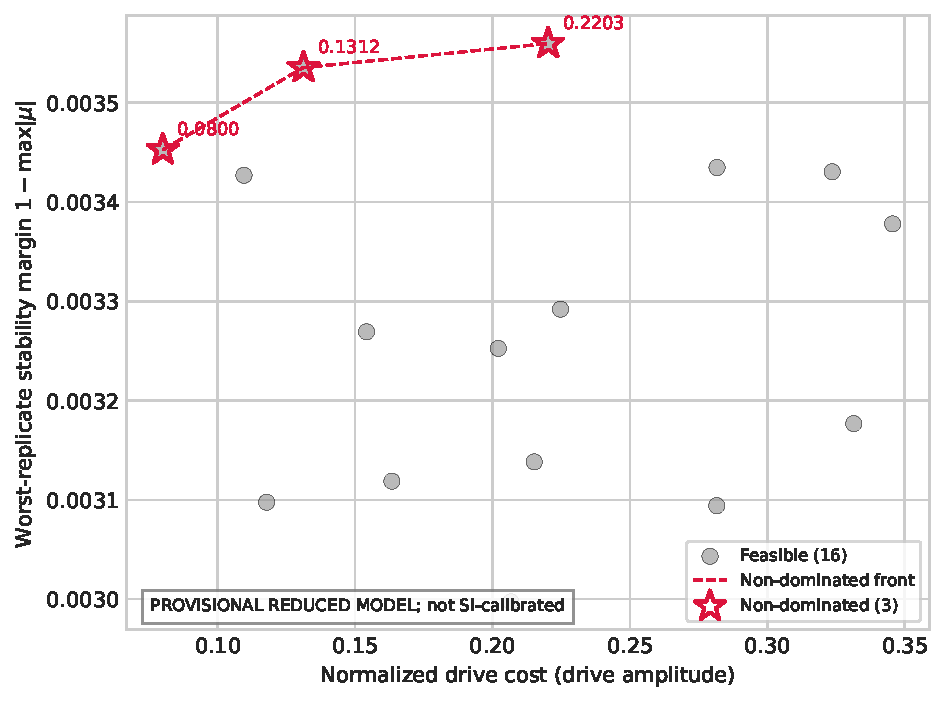
\includegraphics[width=0.72\textwidth,alt={Scatter of sixteen feasible candidates of the reduced adiabatic model in normalized drive cost versus worst-replicate stability margin, with the three non-dominated candidates marked by crimson stars and joined by a dashed front. The front trades increasing drive cost for increasing stability margin. Model-level only.}]{../figures/reduced_model_pareto_v4.pdf}
  \caption{Reduced-model (adiabatic) two-objective Pareto front. Sixteen
  feasible candidates (gray) in normalized drive cost versus worst-replicate
  stability margin $1-\max|\mu|$; the three non-dominated candidates (crimson
  stars, joined by the dashed front) are the points listed in
  \Cref{tab:si-reduced-pareto}. Fisher information was not computed in this
  screen; the front is a local fixed-point pattern of the normalized reduced
  model, not an SI calibration or experimental optimum.}
  \label{fig:si-reduced-pareto}
\end{figure}

\section{Amplitude-quadrature noise model cross-check}
\label{sec:noise-model-crosscheck}

The measured record is $y=X_a+\nu_{\rm det}$ with $X_a=\Re(\alpha)$ the
amplitude quadrature $(a+a^\dagger)/2$, whose vacuum variance is $1/4$. The
Langevin diffusion coefficient that reproduces the quantum master equation for
this quadrature is therefore $\kappa/4$ per amplitude quadrature, not
$\kappa/2$ (the latter is the diffusion of the \emph{normalized} quadrature
$(a+a^\dagger)/\sqrt2$, whose vacuum variance is $1/2$). We verified this
normalization directly on the isolated optical sector of the reference point
(the driven damped linear cavity, $g_1=g_2=0$): the truncated-Fock master
equation~\cite{walls2008,gardiner1985} ($H=-\Delta a^\dagger a+E(a+a^\dagger)$, Lindblad $\sqrt{\kappa}\,a$)
gives $\mathrm{Var}[(a+a^\dagger)/2]=\num{0.25}$, while the Langevin amplitude
with noise $\kappa/2$ gives $\num{0.49}$ (a factor $2$ high) and with
$\kappa/4$ gives $\num{0.245}$ (agreement below $\SI{2}{\percent}$). The mechanical thermal
diffusion is correspondingly $\gamma_j(2n_{\rm th}+1)/4$ per amplitude
quadrature. With these strengths the noise-only floor of the measured record
is $\approx\num{0.25}$ and the strong-coupling observability ratios are
$\num{7.6}$--$\num{17.0}\times$ the floor. The cross-check is recorded in
\texttt{results/langevin\_master\_crosscheck.json} (generator
\texttt{scripts/langevin\_master\_crosscheck.py}).

\section{Interpretation}

The anchored set defines a \emph{reference} operating region, not a validated
device calibration: $\omega_2$ is assumed near-degenerate with $\omega_m$ pending a
two-resonator measurement, $J_m$ must be scanned rather than fixed, and the drive
amplitude and detuning remain model-level coordinates. Any result computed at the
anchored values therefore carries the same
\emph{provisionally-calibrated} status as the reduced-model analysis of the main text
and should not be presented as an experimental optimum.

Placing the strong-coupling hyperchaos regime against the anchors quantifies
the reachability bound: the optomechanical couplings
$g_1/\omega_m=\num{0.3}$ and $g_2/\omega_m=\num{0.27}$ are $\num{2542}\times$ and
$\num{2288}\times$ the anchored $g_0/\omega_m=\num{1.18e-4}$, and the mechanical
damping $\gamma_m/\omega_m=\num{0.02}$ is $\num{720}\times$ the anchored
$\num{2.78e-5}$; the inter-resonator hopping $J_m/\omega_m=\num{0.08}$ is within
the Mathew scan range. The limiting coordinate is the coupling
($\num{2542}\times$). The hyperchaos regime is therefore a model-level
demonstration, not a prediction for the anchored device; the drive amplitude is
not convertible to an input power without the pump frequency and external
coupling, which neither anchor provides.

\bibliography{Chaos_Floquet_SyntheticFlux}

\end{document}
